\section{BROS kết hợp văn bản và vị trí}
BROS kết hợp nội dung chữ với quan hệ vị trí tương đối giữa các vùng chữ trên tài liệu \parencite{hong2022}. Khác RoBERTa, mô hình có thể sử dụng dấu hiệu một số tiền nằm bên phải hay bên dưới một nhãn. BROS không dùng nhánh đặc trưng ảnh, nhưng vẫn cần văn bản và vùng bao làm đầu vào.

\begin{figure}[htbp]
\centering
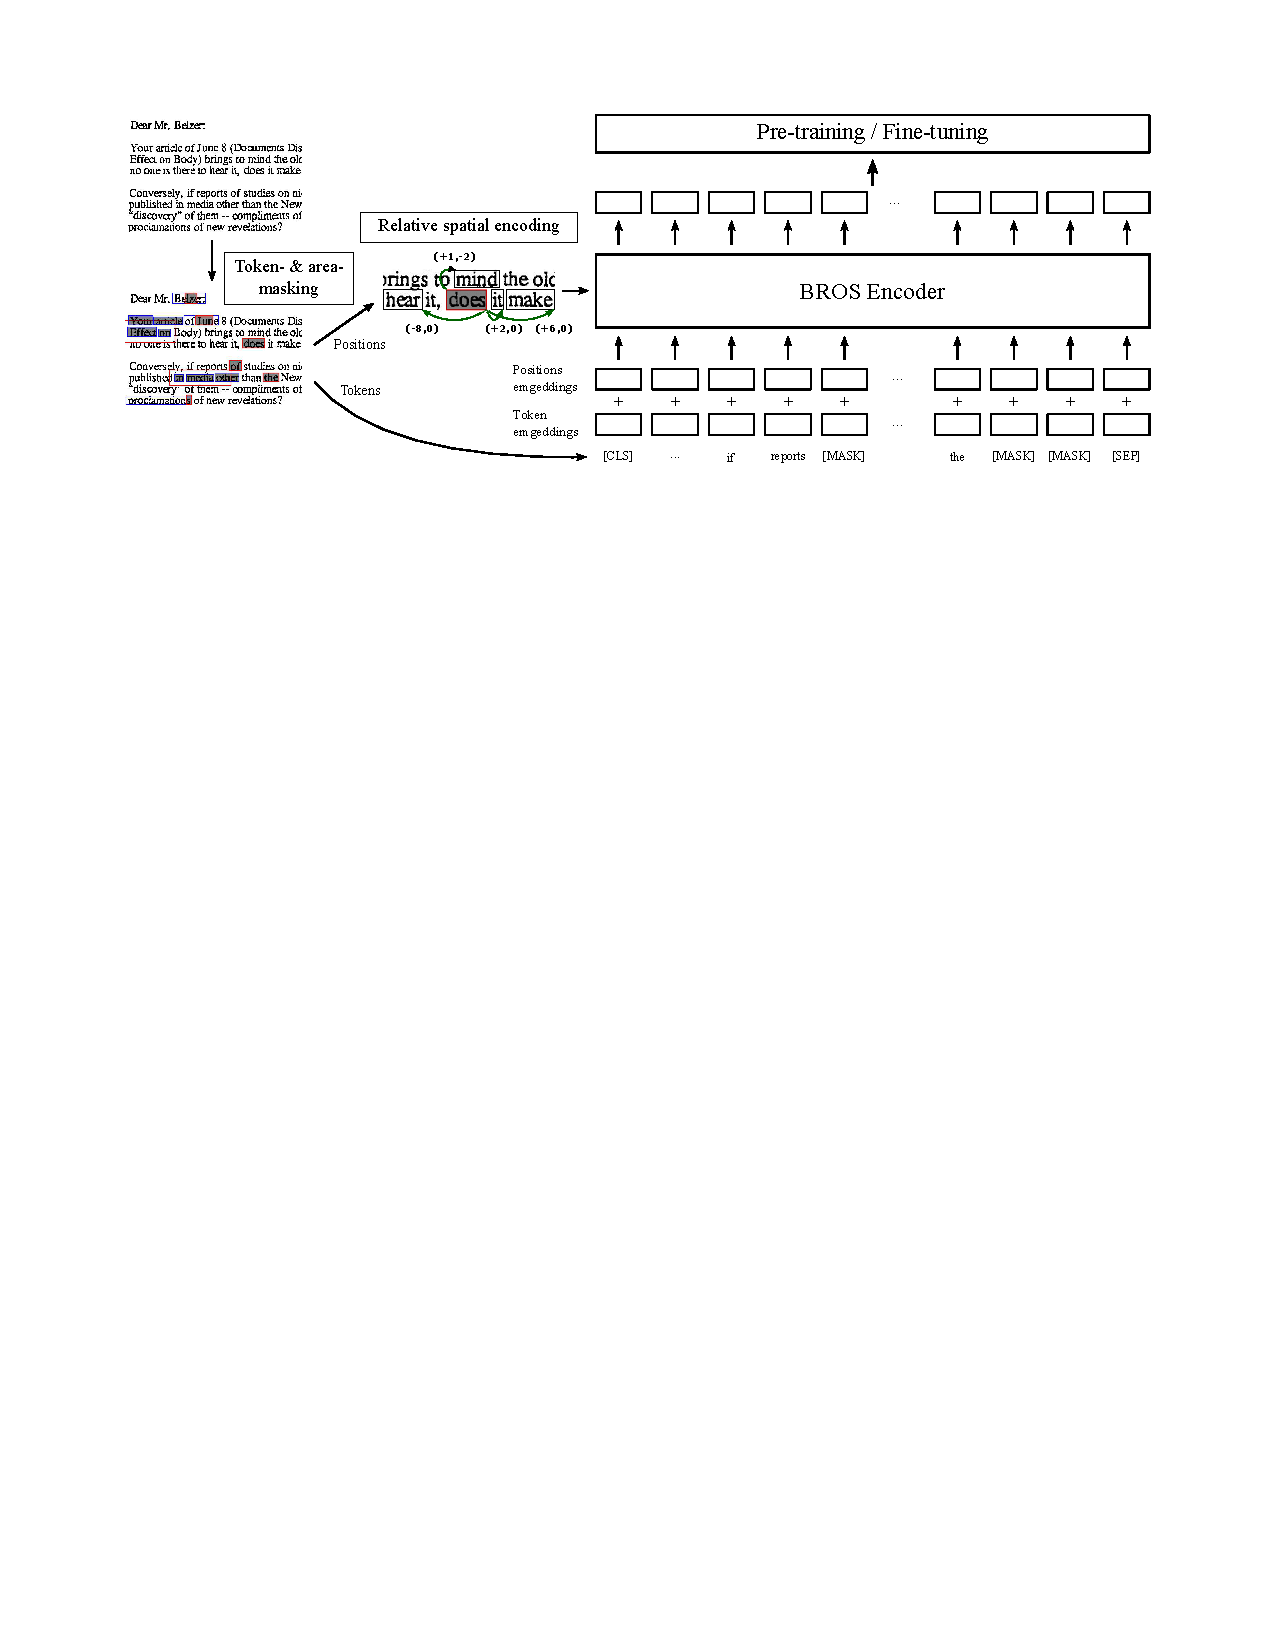
\includegraphics[width=\textwidth]{picture/bros-paper-figure-2.pdf}
\caption{Kiến trúc BROS và các mục tiêu tiền huấn luyện}
\label{fig:bros-original}
\par\centering (Nguồn: \parencite{hong2022})
\end{figure}

Hình~\ref{fig:bros-original} trình bày cơ chế kết hợp chữ và bố cục. BROS mã hóa chênh lệch tọa độ giữa các vùng chữ và đưa quan hệ này vào attention. Ví dụ, hai số tiền có cùng nội dung vẫn có thể nhận biểu diễn khác nhau khi nằm ở cột đơn giá và vùng tổng thanh toán.

Trong tiền huấn luyện, tác giả sử dụng che token và che cả vùng chữ để mô hình học từ ngữ cảnh văn bản lẫn bố cục \parencite{hong2022}. Nhóm nạp trọng số đã có và fine-tune đầu phân loại BIO; không thực hiện lại giai đoạn tiền huấn luyện này.

Bản thực nghiệm dùng BROS với đầu phân loại token, không triển khai bộ liên kết thực thể SPADE được khảo sát trong bài gốc. Vì vậy, các kết quả về khả năng xử lý thứ tự đọc của BROS kết hợp SPADE không được xem là kết quả của nhóm. Giới hạn chính của cấu hình đang dùng là chất lượng chữ, độ chính xác vùng bao và độ dài tối đa 512 token.
